% main.tex: A Hypothesis Engine over History.
%
% Load order matters: biblatex, then hyperref, then bucket.sty. bucket.sty
% conditionally loads cleveref, and cleveref must come after hyperref, so
% hyperref has to load first. See papers/PAPER-STANDARDS.md for the full
% convention this file follows, and papers/template/main.tex for the
% reference build.
\documentclass[11pt]{article}

\usepackage[margin=1in]{geometry}
\usepackage[T1]{fontenc}
\usepackage{csquotes}

\usepackage[backend=biber,style=numeric,sorting=none,maxnames=6,minnames=1]{biblatex}
\addbibresource{refs.bib}
\addbibresource{../bib/common.bib}

\usepackage{hyperref}

\usepackage{bucket} % amsthm envs, \term/\glossentry, cleveref-or-fallback, colors
\usepackage{longtable} % Appendix B's 26-row bead table

\hypersetup{
  colorlinks = true,
  linkcolor  = bucketblue,
  citecolor  = bucketblue,
  urlcolor   = bucketblue,
}

% ---------------------------------------------------------- glossary data --
% papers/history-hypothesis-engine/glossary.tex
%
% Every \glossentry declared here backs a \term{key}{...} call in main.tex.
% \input this file from the preamble, before \begin{document}, per
% papers/PAPER-STANDARDS.md's rule that a \glossentry can be declared
% anywhere before \printglossaryentry runs.
%
% None of these terms has a canon page on bucket.foundation yet: the engine
% they name is a design that has not shipped as a feature of the live
% site. Every URL
% below points instead at the repository path and section of the intake
% specification that defines the term, per this paper's brief ("a link to
% its canon definition on bucket.foundation when one exists, else the repo
% path of the spec section that defines it").

\newcommand{\bktrepo}{https://github.com/bucket-foundation/bucket-foundation/blob/main}

\glossentry{astronomical-year}{astronomical year axis}%
  {\bktrepo/_intake/hypothesis-engine/TIMELINE-AND-COMBINATORICS-SPEC.md\#1-timeline-data-structure}%
  {The engine's time axis: a signed integer line with year 0 present and no
   gap between 1~BCE and 1~CE, unlike the historical BC/AD count. Every
   calendar system maps onto this axis through a converter; see
   \Cref{def:interval}.}

\glossentry{interval-uncertainty}{interval with uncertainty}%
  {\bktrepo/_intake/hypothesis-engine/TIMELINE-AND-COMBINATORICS-SPEC.md\#1-timeline-data-structure}%
  {A dated interval on the astronomical-year axis carrying a distribution
   over its start and end, of type point, uniform, normal, or an OxCal
   posterior with its sampled density curve. \Cref{def:interval}.}

\glossentry{allen-relation}{Allen relation}%
  {\bktrepo/_intake/hypothesis-engine/TIMELINE-AND-COMBINATORICS-SPEC.md\#1-timeline-data-structure}%
  {One of the thirteen qualitative relations between two intervals on a
   time axis (before, meets, overlaps, starts, finishes, during, equals,
   and their inverses) \autocite{allen1983interval}. The engine's only
   vocabulary for ordering a pair of dated hypotheses. \Cref{def:allen}.}

\glossentry{concept-slot}{concept and slot}%
  {\bktrepo/_intake/hypothesis-engine/TIMELINE-AND-COMBINATORICS-SPEC.md\#2-concept-ontology}%
  {A slot (ACTOR, ACTION, OBJECT, PLACE, TIME\_BIN, MECHANISM, or RELATION)
   names one axis of a hypothesis; a concept is one member of a slot's
   vocabulary, carrying its own editable prior log-odds. \Cref{def:slot}.}

\glossentry{prior-logit}{prior logit}%
  {\bktrepo/_intake/hypothesis-engine/TIMELINE-AND-COMBINATORICS-SPEC.md\#2-concept-ontology}%
  {The log-odds a concept node carries before any hypothesis built from it
   sees evidence, a stored, editable number rather than a constant buried
   in code. \Cref{def:slot}.}

\glossentry{other-slot}{open-world slot}%
  {\bktrepo/_intake/hypothesis-engine/IDEAL-STATE-AND-UNKNOWNS-SPEC.md\#6-unknown-unknowns}%
  {A reserved \texttt{OTHER} concept in every slot's vocabulary, carrying a
   Dirichlet-process new-concept probability mass so a hypothesis can name
   an actor, action, or mechanism the ontology has not yet added.
   \Cref{sec:unknowns}.}

\glossentry{placement-hypothesis}{placement hypothesis}%
  {\bktrepo/_intake/hypothesis-engine/TIMELINE-AND-COMBINATORICS-SPEC.md\#3-the-combinatorial-function}%
  {A hypothesis of the form "event $E$ happened in interval $T$," one point
   in the product space $H = \text{ACTOR} \times \text{ACTION} \times
   \text{OBJECT} \times \text{PLACE} \times \text{TIME\_BIN} \times
   \text{MECHANISM}$. \Cref{def:placement}.}

\glossentry{sequence-hypothesis}{sequence hypothesis}%
  {\bktrepo/_intake/hypothesis-engine/TIMELINE-AND-COMBINATORICS-SPEC.md\#3-the-combinatorial-function}%
  {A hypothesis of the form "$E_1$ then $E_2$," one point in $H_{\mathrm{seq}}
   = H \times \text{ALLEN\_RELATION} \times H$: two placements joined by one
   of the thirteen Allen relations. \Cref{def:sequence}.}

\glossentry{address}{hypothesis address}%
  {\bktrepo/_intake/hypothesis-engine/TIMELINE-AND-COMBINATORICS-SPEC.md\#3-the-combinatorial-function}%
  {The prime-factorization identifier of a hypothesis: each slot's
   vocabulary index plus one becomes the exponent of a fixed prime, and the
   product is the hypothesis's integer ID, decodable by trial division
   alone. \Cref{def:address}.}

\glossentry{evidence-kind}{evidence kind}%
  {\bktrepo/_intake/hypothesis-engine/TIMELINE-AND-COMBINATORICS-SPEC.md\#4-truth-score-as-additive-prime-knowledge}%
  {One of nine independent modalities evidence can carry: material or
   archaeological, textual or documentary, genetic, linguistic, astronomical
   or radiometric, geological or climate, oral tradition or myth,
   iconographic, or model-based inference. \Cref{def:evidence}.}

\glossentry{evidence-tier}{evidence tier}%
  {\bktrepo/_intake/hypothesis-engine/HISTORY-HYPOTHESIS-ENGINE-SPEC.md\#2-truth-score-model}%
  {A source-reliability band, T1 through T6, mapped from a source-quality
   score and carrying a fixed weight $k(\text{tier})$ from $2.0$ down to
   $0.1$, the maximum log-odds swing one independent piece of evidence at
   that tier contributes. \Cref{def:evidence}.}

\glossentry{evidence-span}{evidence span}%
  {\bktrepo/_intake/hypothesis-engine/HISTORY-HYPOTHESIS-ENGINE-SPEC.md\#3-hypothesis-data-model}%
  {The character range and named field (\texttt{who}, \texttt{what},
   \texttt{when}, \texttt{where}, \texttt{why}, or \texttt{causal\_direction})
   an evidence item supports, grounding a claim at the field level rather
   than the hypothesis as a whole. \Cref{def:evidence}.}

\glossentry{opinion}{opinion}%
  {\bktrepo/_intake/hypothesis-engine/IDEAL-STATE-AND-UNKNOWNS-SPEC.md\#2-belief-as-opinion}%
  {A subjective-logic tuple $\omega = (b, d, u, a)$, belief, disbelief,
   uncertainty mass, and base rate, with $b + d + u = 1$
   \autocite{josang2016subjective}, replacing a single posterior score.
   \Cref{def:opinion}.}

\glossentry{projected-probability}{projected probability}%
  {\bktrepo/_intake/hypothesis-engine/IDEAL-STATE-AND-UNKNOWNS-SPEC.md\#2-belief-as-opinion}%
  {The scalar read-out $P(h) = b(h) + a(h) \cdot u(h)$ of an opinion,
   collapsing belief, disbelief, and uncertainty mass into one number for
   ranking while the opinion itself keeps the three apart.
   \Cref{def:projection}.}

\glossentry{base-rate}{base rate}%
  {\bktrepo/_intake/hypothesis-engine/IDEAL-STATE-AND-UNKNOWNS-SPEC.md\#2-belief-as-opinion}%
  {An opinion's resting point under total ignorance, $a(h) =
   \operatorname{sigmoid}(L_{\mathrm{prior}}(h))$: what $P(h)$ equals when
   $b = d = 0$ and $u = 1$. \Cref{def:opinion}.}

\glossentry{stemma}{stemma}%
  {\bktrepo/_intake/hypothesis-engine/IDEAL-STATE-AND-UNKNOWNS-SPEC.md\#3-source-dependence}%
  {A dependency graph over evidence sources, one node per source and a
   directed \texttt{copies\_from} or \texttt{shares\_archetype\_with} edge
   with a copy-confidence weight, borrowed from manuscript philology.
   \Cref{def:stemma}.}

\glossentry{effective-count}{effective count}%
  {\bktrepo/_intake/hypothesis-engine/IDEAL-STATE-AND-UNKNOWNS-SPEC.md\#3-source-dependence}%
  {$n_{\mathrm{eff}}$, the count of connected components in a stemma after
   pruning low-confidence edges, replacing the raw count of evidence
   clusters everywhere a diminishing-returns discount is applied.
   \Cref{def:stemma}.}

\glossentry{detectability}{detectability}%
  {\bktrepo/_intake/hypothesis-engine/IDEAL-STATE-AND-UNKNOWNS-SPEC.md\#4-preservation-and-detectability}%
  {$\delta(\mathrm{period}, \mathrm{medium}, \mathrm{region}) \in [0,1]$,
   the probability that evidence of a true hypothesis would have survived
   and been found in that period, medium, and region; scales absence
   evidence rather than treating it at a flat weight. \Cref{def:detect}.}

\glossentry{gap-node}{gap node}%
  {\bktrepo/_intake/hypothesis-engine/IDEAL-STATE-AND-UNKNOWNS-SPEC.md\#5-known-unknowns-as-gap-nodes}%
  {A first-class node for something the corpus has not yet looked at, an
   unexcavated site, an untranslated text, an undated stratum, an unread
   archive, naming the hypotheses it would move and its expected value of
   information. \Cref{def:gap}.}

\glossentry{voi-score}{value of information}%
  {\bktrepo/_intake/hypothesis-engine/IDEAL-STATE-AND-UNKNOWNS-SPEC.md\#5-known-unknowns-as-gap-nodes}%
  {A gap node's ranking score, folding expected uncertainty reduction,
   novelty, coverage gap, historical gap, and provider disagreement into
   one number that orders the active-learning queue. \Cref{def:gap}.}

\glossentry{missing-mass}{missing mass}%
  {\bktrepo/_intake/hypothesis-engine/IDEAL-STATE-AND-UNKNOWNS-SPEC.md\#6-unknown-unknowns}%
  {The Good-Turing estimate $f_1/N$ of the unseen share of the hypothesis
   space, where $f_1$ is the count of hypotheses observed in exactly one
   generation run and $N$ is the total observed across runs.
   \Cref{def:missingmass}.}

\glossentry{chao1}{Chao1 estimator}%
  {\bktrepo/_intake/hypothesis-engine/IDEAL-STATE-AND-UNKNOWNS-SPEC.md\#6-unknown-unknowns}%
  {The richness estimator $S_{\mathrm{est}} = S_{\mathrm{obs}} +
   f_1^2/(2f_2)$, sizing the total hypothesis or evidence count from how
   many items were seen exactly once or twice across repeated runs
   \autocite{colwell1994estimating,chao1987estimating}. \Cref{def:missingmass}.}

\glossentry{coverage-share}{coverage share}%
  {\bktrepo/_intake/hypothesis-engine/IDEAL-STATE-AND-UNKNOWNS-SPEC.md\#8-coverage-claim}%
  {The fraction $\mathrm{hypotheses\_generated\_and\_scored}(\mathrm{bin}) /
   S_{\mathrm{est}}(\mathrm{bin})$ reported with a confidence interval per
   time bin, replacing the claim that generation produces the full set.
   \Cref{sec:unknowns}.}

\glossentry{surprise-event}{surprise event}%
  {\bktrepo/_intake/hypothesis-engine/IDEAL-STATE-AND-UNKNOWNS-SPEC.md\#6-unknown-unknowns}%
  {A logged event when new evidence matches no hypothesis address the
   generator has materialized at any slot-value combination; its rate,
   tracked per period, is a health signal on whether the ontology has
   fallen behind the evidence. \Cref{sec:unknowns}.}

\glossentry{prior-profile-robustness}{prior-profile robustness}%
  {\bktrepo/_intake/hypothesis-engine/IDEAL-STATE-AND-UNKNOWNS-SPEC.md\#6-unknown-unknowns}%
  {$1$ minus the spread of $P(h)$ across four prior profiles, consensus,
   skeptic, fringe, and uniform; a hypothesis whose rank flips depending on
   which profile scores it earns less trust than one that does not.
   \Cref{sec:unknowns}.}

\glossentry{target-blind}{target-blind generation}%
  {\bktrepo/_intake/hypothesis-engine/IDEAL-STATE-AND-UNKNOWNS-SPEC.md\#7-the-model-accounting-for-itself}%
  {The rule that hypothesis generation stays complete and scored the same
   way regardless of which target reading, orthodox, fringe, or any
   consensus status between, a hypothesis would end up supporting; the
   history engine's own name for QAD's quantum-blind rule.
   \Cref{sec:engine-loop}.}

\glossentry{ranking-tournament}{ranking tournament}%
  {\bktrepo/_intake/hypothesis-engine/HISTORY-HYPOTHESIS-ENGINE-SPEC.md\#5-hypothesis-generation-loop}%
  {The Elo-seeded, pairwise-debate ranking pass over the generated
   frontier, seeded from each hypothesis's posterior and recomputed against
   the belief model every fixed number of rounds. \Cref{sec:engine-loop}.}

\glossentry{self-report}{self-report}%
  {\bktrepo/_intake/hypothesis-engine/IDEAL-STATE-AND-UNKNOWNS-SPEC.md\#7-the-model-accounting-for-itself}%
  {A corpus artifact every generation run emits: its assumptions, which
   slot vocabularies it judged incomplete, its missing-mass estimate, and
   its calibration score against the holdout tests.
   \Cref{sec:engine-loop}.}

\glossentry{retrieval-envelope}{retrieval envelope}%
  {\bktrepo/_intake/hypothesis-engine/HISTORY-HYPOTHESIS-ENGINE-SPEC.md\#8-implementation-plan}%
  {An immutable record of one fetch, linked to a \texttt{RetrievalRun} id,
   so a later re-fetch cannot silently change what an earlier run found
   without a new run id appearing in the provenance chain.
   \Cref{sec:engine-loop}.}

\glossentry{neighbor-mutation}{neighbor mutation}%
  {\bktrepo/_intake/hypothesis-engine/TIMELINE-AND-COMBINATORICS-SPEC.md\#3-the-combinatorial-function}%
  {The evolver's one-slot mutation move: from a hypothesis $h$, hold every
   slot fixed but one and range that slot over its vocabulary, yielding
   every hypothesis address one edit away from $h$. \Cref{def:neighbors}.}

\glossentry{founder-review}{founder review}%
  {\bktrepo/_intake/hypothesis-engine/HISTORY-HYPOTHESIS-ENGINE-SPEC.md\#7-human-review-budget}%
  {A weekly-budgeted queue of hypotheses whose posterior falls inside a
   contested band or that touch a high-impact claim; a founder verdict
   enters as one evidence kind at the top tier, folded by fusion rather
   than overriding it. \Cref{sec:calibration}.}


% ------------------------------------------------------- Lean listing helper --
% Every Lean file this appendix cites is being written in parallel under
% lean/Bucket/ (see papers/PAPER-STANDARDS.md's Lean rule and this paper's
% own Section 12). \IfFileExists guards each \lstinputlisting so a pass
% run before a given file lands still compiles: it prints the identifier
% names that file will carry instead of failing the build.
% #1 = lean-snapshots/<Name>.lean, an ASCII-safe transliteration built by
% make_lean_snapshots.py from the real lean/Bucket/<Name>.lean (Lean 4
% source is Unicode throughout; this toolchain's listings has no
% listingsutf8 and no Unicode math font, so the real file cannot go
% through \lstinputlisting directly, see make_lean_snapshots.py's own
% header). #2 = the real source path, shown in the pending note only.
% #3 = the Lean identifier names #1 will define.
\newcommand{\bucketlean}[3]{%
  \IfFileExists{#1}{%
    \lstinputlisting[style=bucketlean]{#1}%
  }{%
    \par\noindent{\footnotesize\ttfamily\color{bucketgray}
    -- \texttt{#2}: pending; will define \texttt{#3}.\par}%
  }%
}

\title{A Hypothesis Engine over History: Combinatorial Generation,\\
  Subjective-Logic Belief, and Structural Unknowns}
\author{Gianangelo Dichio \\ Bucket Foundation}
\date{2026-09-09}

\begin{document}
\maketitle

\begin{abstract}
History accumulates claims faster than any framework scores them: a
correlation, a dated fragment, a contested attribution each carry their
own confidence number, with no credence a reader can compare across
hypotheses. We present a design for a hypothesis engine that treats every
placement of an actor, action, and mechanism into a dated interval, and
every ordered pair of placements, as one point in a combinatorial address
space, generated whether or not the literature supports it. Each
hypothesis carries a subjective-logic opinion, belief, disbelief, and
uncertainty mass, rather than one point estimate, so a hypothesis nobody
has examined reads apart from one refuted. A structural-unknowns layer
puts the engine's blind spots, an unnamed concept, an unexcavated gap,
undiscovered evidence, inside the model instead of a footnote added
later. We derive the address scheme's size and injectivity, the opinion
model's normalization and probability bound, and lay out an engine loop
of generation, critique, ranking, and evolution, checked against a
sibling engine for a different corpus. We close with a calibration
design, two holdout tests and two candidate pilot periods, naming what in
the model stays uncalibrated. No results are claimed here; this is a
design and the proofs that check it.
\end{abstract}

\section{Introduction}
\label{sec:intro}

A corpus of historical claims grows by accretion: a correlation between
two flood myths, a radiocarbon date on a construction fill, a contested
reading of an inscription. Four disjoint scores can sit on such a claim,
an embedding similarity, a source-quality heuristic, a tier-classifier
softmax, a keyword count, and none answers the question a reader asks:
how likely is this account of the past to be true. Closing that gap
raises three problems at once, and a design that solves only one of them
does not close it.

First, the set of hypotheses worth scoring cannot be bounded by what
published sources already argue. A corpus with a coherent radiocarbon date
and a coherent construction technique supports the reading that farmers
built a shrine at a Neolithic site; the same corpus, read against the same
address space, also supports the reading that an unnamed actor with an
unnamed mechanism did it, at a prior so low no scholar would publish it
and no engine should refuse to name it. An engine that only proposes what
a literature review would propose inherits that literature's blind spots
along with its evidence.

Second, a posterior collapsed to one number cannot tell a reader whether
a hypothesis sits at even odds because two strong, opposed evidence
clusters cancel, or because nobody has looked. A sigmoid score $\tau \in
[0,1]$ answers both cases with the same number near $0.5$. A reader
deciding whether to go dig, translate, or read needs the model to state
which case it is in.

Third, a generator that only reports on the hypotheses it materializes has
no account of what it has not materialized. A closed vocabulary of actors,
mechanisms, and places has no address for a concept nobody has named yet;
a hypothesis space with $10^{24}$ points has no process that visits all of
it; a claim of "the full set" over a space that large is a claim no
process on file can back.

This paper answers each problem with one piece of machinery, over
Sections~\ref{sec:timeline} through~\ref{sec:calibration}, and derives the
part of each piece that can be derived rather than measured. The five
contributions are:

\begin{enumerate}
  \item A combinatorial \term{address}{address} scheme, a fixed-prime
    factorization over a hypothesis's slot vocabulary, that names every
    \term{placement-hypothesis}{placement} and
    \term{sequence-hypothesis}{sequence} hypothesis a corpus's vocabulary
    can express, decodable by trial division alone, without materializing
    the space it addresses (\Cref{sec:combinatorics}).
  \item A subjective-logic \term{opinion}{opinion} model that carries
    belief, disbelief, and uncertainty mass apart from one another, proved
    to sum to one and to project to a probability in $[0,1]$, reducing to
    the corpus's existing sigmoid posterior at the limit of total ignorance
    (\Cref{sec:belief}).
  \item A structural-unknowns layer, \term{gap-node}{gap nodes} ranked by
    \term{voi-score}{value of information}, \term{other-slot}{open-world
    slots}, \term{missing-mass}{missing-mass} estimation, and
    \term{prior-profile-robustness}{prior-profile robustness}, that gives
    the engine's own blind spots a place in the model rather than a
    footnote a human adds later (\Cref{sec:unknowns}).
  \item An engine loop, generation, critique, \term{ranking-tournament}{
    ranking tournament}, evolution, and \term{self-report}{self-report},
    adapted from the AI co-scientist pattern
    \autocite{gottweis2025coscientist} and cross-walked line by line
    against \texttt{scientific-discovery}, a sibling engine built for a
    different corpus and cited throughout as a software repository
    rather than a published article (\Cref{sec:engine-loop}).
  \item A calibration design, two holdout splits and two candidate pilot
    periods stated as design options with no result claimed, naming the
    constants this engine still runs on uncalibrated instead of leaving
    them hidden (\Cref{sec:calibration}).
\end{enumerate}

\section{Related work}
\label{sec:related}

This section places each of the five contributions of \Cref{sec:intro}
against the closest published system it extends, departs from, or
stands in for.

\paragraph{AI hypothesis generation.} A generate, critique, rank, evolve
loop over a claims graph, with Elo seeded from a Bayesian posterior and
updated by simulated debate, is the shape DeepMind's AI co-scientist runs
over biomedical literature \autocite{gottweis2025coscientist};
\Cref{sec:engine-loop} follows the same shape over historical correlations.
AlphaEvolve mutates a program population against a programmatic fitness
function \autocite{novikov2025alphaevolve}, generalizing FunSearch's
evolution of one function toward a numeric objective
\autocite{romeraparedes2024funsearch}; neither has a crisp fitness
function for a qualitative historical claim, so \Cref{sec:belief}'s
belief model stands in its place. Sakana's AI Scientist runs an
idea-to-code-to-experiment-to-paper-draft loop scored by an automated
reviewer \autocite{lu2024aiscientist}; its v2 successor replaces that
loop with an agentic tree search and submitted three fully autonomous
manuscripts to a peer-reviewed ICLR workshop, one of which cleared the
human acceptance threshold \autocite{yamada2025aiscientistv2}. Stanford's
Virtual Lab specializes agent roles under a principal-investigator agent
and budgets a small human-review pass over its output
\autocite{swanson2024virtuallab}, the pattern \Cref{sec:calibration}'s
\term{founder-review}{founder-review} budget reuses. MIT's SciAgents
walks a roughly thousand-paper graph with ontologist, scientist, and
critic roles \autocite{ghafarollahi2024sciagents}, the role-specialization
pattern \Cref{sec:engine-loop} extends with an unknown-unknown generator
and a preservation critic. FutureHouse's Robin closes a
literature-to-hypothesis-to-experiment loop against a real wet-lab
result, validating one candidate, ripasudil, for dry age-related macular
degeneration and generating hypotheses across ten additional diseases
\autocite{ghareeb2025robin}; with no wet lab to close against,
\Cref{sec:calibration}'s holdout splits stand in. MC-NEST extends Monte
Carlo tree search with an explicit explore or exploit control and an LLM
judge scoring novelty, clarity, significance, and verifiability
\autocite{rabby2024mcnest}, the control \Cref{sec:engine-loop}'s ranking
tournament borrows.

\paragraph{Belief representation.} Dempster and Shafer's theory of
evidence assigns belief mass to subsets of a hypothesis space rather than
to single outcomes \autocite{dempster1967upper,shafer1976mathematical};
Jøsang's subjective logic specializes that theory to a single binomial
opinion $(b, d, u, a)$ with an explicit uncertainty mass and a closed-form
cumulative fusion rule \autocite{josang2016subjective}, the exact form
\Cref{sec:belief} builds the engine's posterior on top of.

\paragraph{Chronology.} Bronk Ramsey's Bayesian phase modeling over
stratigraphy and the radiocarbon calibration curve, the method behind the
OxCal program, turns a set of dated observations into a posterior density
over a period's true date \autocite{bronkramsey2009bayesian}; Allen's
thirteen qualitative interval relations give the vocabulary for ordering
two such dated periods without committing to exact dates
\autocite{allen1983interval}. \Cref{sec:timeline} builds the timeline
substrate on both.

\paragraph{Computational history.} Ithaca restores, dates, and places
damaged ancient inscriptions as ranked, evidence-grounded hypotheses,
trained on 176,861 inscriptions and validated against 23 historians
\autocite{assael2022ithaca}; Aeneas extends the same approach to
contextualizing and attributing longer passages of ancient text
\autocite{assael2025aeneas}. Both ground a hypothesis in retrieved
primary evidence with a stated confidence, the pattern \Cref{sec:belief}'s
evidence items carry forward. Seshat codes complex societies into a
per-polity, per-century variable databank built for testing theories of
social evolution \autocite{turchin2015seshat}; a recent benchmark on that
databank, referred to throughout the intake specification this paper
implements as Hist-LLM, reports current language models near 46 percent
recall on Seshat's coded judgments
(\texttt{IDEAL-STATE-AND-UNKNOWNS-SPEC.md} \S7). That benchmark has no
resolvable DOI or arXiv identifier, so it is not a bibliography entry
here; \Cref{sec:engine-loop} and \Cref{sec:limitations} cite its finding
by pointing at the specification section that reports it, the rule this
paper's glossary also follows for a term with no external citable
source.

\paragraph{Species-richness estimators.} Good's population-frequency
estimator gives the unseen share of a sampled population as $f_1/N$, the
count of once-seen classes over the total sample
\autocite{good1953population}; Colwell and Coddington's extrapolation
review restates that estimator's richness form, commonly called Chao1,
as $S_{\mathrm{est}} = S_{\mathrm{obs}} + f_1^2/(2f_2)$
\autocite{colwell1994estimating}, building on Chao's own capture-recapture
estimator for sparse observation data \autocite{chao1987estimating}.
\Cref{sec:unknowns} applies both to a generator's own output instead of a
sampled ecological population.

\paragraph{Dirichlet process.} Ferguson's nonparametric prior over an
unbounded set of categories gives a closed-form probability that the next
draw names a category not yet seen, $\alpha/(\alpha+N)$
\autocite{ferguson1973bayesian}; \Cref{sec:unknowns}'s open-world slot
reserves exactly this mass for a concept the ontology has not yet added.

\paragraph{Gödel numbering.} Gödel's proof that a formal system's own
statements can be arithmetized as numbers, decodable by the fixed
factorization of a fixed base sequence \autocite{godel1931unentscheidbare},
is the same move \Cref{sec:combinatorics}'s address scheme makes over a
hypothesis's slot values in place of a formula's symbols.

\paragraph{Sibling engine.} \texttt{scientific-discovery}
(\url{https://github.com/gianyrox/quantum-algorithm-discovery}, v0.11) is
a software repository with no DOI, arXiv identifier, or Zenodo archive
attached; per \texttt{papers/PAPER-STANDARDS.md}'s citation rule it is
cited here by URL rather than entered into the bibliography. It
retrieves papers, extracts a derived research object from each, searches
for structural families across disciplines, and maps surviving families
against known quantum algorithms. The history engine runs the same
four-stage shape, retrieve, extract, search, target, over a claims graph
instead of a paper corpus; \texttt{CROSSWALK-QUANTUM-ALGORITHM-
DISCOVERY.md} works the correspondence module by module, and
Sections~\ref{sec:unknowns} and~\ref{sec:engine-loop} carry forward eight
patterns that crosswalk pulls into this design.

\section{Preliminaries}
\label{sec:prelim}

This section defines every term \Cref{sec:timeline} through
\Cref{sec:calibration} depends on, each linked via
\texttt{\textbackslash term} to a glossary entry (\Cref{app:glossary})
and a Lean counterpart (\Cref{app:lean}). \Cref{tab:symbols} collects
the symbols carried across
every section below as a single reference, so a symbol's meaning does
not have to be traced back through whichever section introduced it.

\begin{table}[htbp]
\centering
\small
\caption{Symbols carried across \Cref{sec:timeline} through
  \Cref{sec:calibration}, with the equation or definition that first
  fixes each.}
\label{tab:symbols}
\begin{tabular}{@{}cl@{}}
  \toprule
  Symbol & Meaning \\
  \midrule
  $a$, $b$, $d$, $u$ & Base rate, belief, disbelief, uncertainty mass of one opinion $\omega(h)$ (\Cref{def:opinion}) \\
  $P$ & Projected probability $P(h) = b(h) + a(h)\,u(h)$ (\Cref{def:projection}) \\
  $r$, $s$ & Pooled supporting and refuting evidence weight for $h$ (\Cref{def:opinion-fusion}) \\
  $W$ & Total-ignorance weight, fixed at $2$ (\Cref{eq:opinion-sum}) \\
  $D(n)$ & Diminishing-returns discount on $n$ corroborating clusters, $\lambda = 0.5$ (\Cref{eq:diminishing}) \\
  $X(K)$ & Cross-kind independence bonus over $K$ evidence kinds (\Cref{eq:cross-kind}) \\
  $\mu$ & The corpus's original contradiction-penalty weight, $0.5$; superseded by \Cref{eq:opinion-sum} \\
  $\delta$ & Detectability, $\delta(\mathrm{period}, \mathrm{medium}, \mathrm{region}) \in [0,1]$ (\Cref{def:detect}) \\
  $\tau$ & The corpus's pre-opinion sigmoid posterior, $\tau = \operatorname{sigmoid}(L)$ (\Cref{sec:intro}) \\
  $L(h)$ & Ranking score, the logit of $P(h)$ shifted by $\Theta_{\mathrm{temporal}}(h)$ (\Cref{eq:rank}) \\
  \bottomrule
\end{tabular}
\end{table}

\begin{definition}[Astronomical-year interval]
\label{def:interval}
The engine's time axis is a signed integer line in astronomical years:
year $0$ exists, and there is no gap between $1$~BCE and $1$~CE the way
the historical BC/AD count has one. An \term{interval-uncertainty}{
interval} $I = (\mathrm{start}, \mathrm{end}, \mathrm{uncertainty})$ pairs
a start and end year with a distribution over each, point, uniform,
normal, or an OxCal-style posterior carrying its own sampled density
curve \autocite{bronkramsey2009bayesian}. The \term{astronomical-year}{
astronomical year axis} sits under every dated node the engine holds.
Lean counterpart: \texttt{Bucket.Timeline.Interval}.
\end{definition}

\begin{definition}[Allen relation]
\label{def:allen}
An \term{allen-relation}{Allen relation} is one of the thirteen
qualitative relations between two intervals $I_1$ and $I_2$:
\textsc{before}, \textsc{after}, \textsc{meets}, \textsc{met-by},
\textsc{overlaps}, \textsc{overlapped-by}, \textsc{starts}, \textsc{
started-by}, \textsc{finishes}, \textsc{finished-by}, \textsc{during},
\textsc{contains}, \textsc{equals} \autocite{allen1983interval}. An edge
between two dated nodes carries exactly one such relation plus a
confidence and a provenance pointer to the date claim it derives from.
Lean counterpart: \texttt{Bucket.Timeline.AllenRelation}.
\end{definition}

\begin{definition}[Concept and slot]
\label{def:slot}
A \emph{slot} is one of \texttt{ACTOR}, \texttt{ACTION}, \texttt{OBJECT},
\texttt{PLACE}, \texttt{TIME\_BIN}, \texttt{MECHANISM}, or
\texttt{RELATION}. A \term{concept-slot}{concept} $c$ is a member of one
slot's vocabulary, carrying a \term{prior-logit}{prior logit}
$\ell(c) \in \mathbb{R}$, a consensus status on the scale
majority-scholarly through non-consensus, and a rationale string. Every
slot's vocabulary carries an \term{other-slot}{\texttt{OTHER}} concept
with reserved probability mass, per \Cref{sec:unknowns}. Lean
counterpart: \texttt{Bucket.Concept.Slot}.
\end{definition}

\begin{definition}[Placement hypothesis]
\label{def:placement}
A \term{placement-hypothesis}{placement hypothesis} is one point in the
product space
\begin{equation}
  \label{eq:placement-space}
  H = \mathtt{ACTOR} \times \mathtt{ACTION} \times \mathtt{OBJECT}
    \times \mathtt{PLACE} \times \mathtt{TIME\_BIN} \times \mathtt{MECHANISM},
\end{equation}
read as the claim that the named actor performed the named action on the
named object at the named place, inside the named time bin, by the named
mechanism. Lean counterpart: \texttt{Bucket.Hypothesis.Placement}, which
carries the full \texttt{Interval} the corpus stores for a placement
rather than the bucketed \texttt{TIME\_BIN} identifier this product
space addresses; \texttt{Bucket.Address.SlotTuple}
(\Cref{sec:combinatorics}) is the Lean structure that names
\texttt{timeBin} as its own field, the one \Cref{eq:address} encodes.
\end{definition}

\begin{definition}[Sequence hypothesis]
\label{def:sequence}
A \term{sequence-hypothesis}{sequence hypothesis} is one point in
\begin{equation}
  \label{eq:sequence-space}
  H_{\mathrm{seq}} = H \times \mathtt{ALLEN\_RELATION} \times H,
\end{equation}
read as two placements joined by one of the thirteen Allen relations of
\Cref{def:allen}. Every causal or co-occurrence hypothesis is a sequence
hypothesis read through a fixed mapping from Allen relation to causal
reading. Lean counterpart: \texttt{Bucket.Hypothesis.Sequence}.
\end{definition}

\begin{definition}[Address]
\label{def:address}
Fix the first thirteen primes $p_1, \ldots, p_{13} = 2, 3, 5, 7, 11, 13,
17, 19, 23, 29, 31, 37, 41$ in slot order, six for a placement, one for
the relation, six more for a sequence's second placement. Index each
slot's vocabulary from $0$. The \term{address}{address} of a slot
assignment is
\begin{equation}
  \label{eq:address}
  \mathrm{address}(\mathrm{slots}) = \prod_{k} p_k^{\,v_k(\mathrm{slots}) + 1},
\end{equation}
where $v_k(\mathrm{slots})$ is the vocabulary index of the value assigned
to the $k$-th slot in the fixed slot order. Lean counterpart:
\texttt{Bucket.Address.encode}.
\end{definition}

\begin{definition}[Evidence item]
\label{def:evidence}
An evidence item is a tuple $(\kappa, \theta, \sigma, \pi, e)$: a
\term{evidence-kind}{kind} $\kappa$ drawn from the nine modalities of
\Cref{sec:belief}, a \term{evidence-tier}{tier} $\theta \in
\{\mathrm{T1}, \ldots, \mathrm{T6}\}$ carrying a fixed weight
$k(\theta)$, a \term{evidence-span}{span} $\sigma$ naming the character
range and hypothesis field it grounds, a provenance record $\pi$ naming
who or what asserted it, and an edge strength $e \in [0, 1]$. An evidence item has no independent Lean type of its own in this pass:
its definitional weight, kind, tier, and strength, is exactly what
\Cref{eq:cluster-weight}'s $s_i = k(\theta_i) \cdot e_i$ reduces it to
before it reaches \texttt{Bucket.Belief.fromEvidence}'s $r$ and $s$
arguments.
\end{definition}

\begin{definition}[Opinion]
\label{def:opinion}
An \term{opinion}{opinion} is a tuple $\omega(h) = (b(h), d(h), u(h),
a(h))$: belief, disbelief, uncertainty mass, and \term{base-rate}{base
rate}, over a hypothesis $h$. Lean counterpart:
\texttt{Bucket.Belief.Opinion}.
\end{definition}

\begin{definition}[Projected probability]
\label{def:projection}
The \term{projected-probability}{projected probability} of an opinion
$\omega(h) = (b, d, u, a)$ is
\begin{equation}
  \label{eq:projection}
  P(h) = b(h) + a(h) \cdot u(h).
\end{equation}
Lean counterpart: \texttt{Bucket.Belief.project}.
\end{definition}

\begin{definition}[Stemma and effective count]
\label{def:stemma}
A \term{stemma}{stemma} over a set of evidence sources is a directed
graph with one node per source and an edge \texttt{copies\_from} or
\texttt{shares\_archetype\_with} carrying a copy-confidence weight in
$[0,1]$. Fix a threshold $\theta_{\mathrm{prune}}$ (default $0.6$); the
\term{effective-count}{effective count} $n_{\mathrm{eff}}$ of a cluster is
the number of connected components of the stemma after removing every
edge below $\theta_{\mathrm{prune}}$. $n_{\mathrm{eff}}$ replaces the raw
cluster count $n$ everywhere a diminishing-returns discount is applied.
No Lean counterpart is named for this pass: connected-component counting
over a pruned stemma graph is not yet formalized, and $n_{\mathrm{eff}}$
reaches \texttt{Bucket.Belief.fromEvidence} only as a plain \texttt{Nat}
substituted for $n$ in \Cref{eq:diminishing} before that function is
called. \Cref{sec:limitations} states this as an open item in the Lean
listings alongside detectability and gap nodes.
\end{definition}

\begin{definition}[Detectability]
\label{def:detect}
\term{detectability}{Detectability} $\delta(\mathrm{period},
\mathrm{medium}, \mathrm{region}) \in [0,1]$ is the probability that
evidence of a true hypothesis would have survived and been found in that
period, medium, and region. No Lean counterpart is named for this pass;
\Cref{sec:limitations} states this as an open item in the Lean listings.
\end{definition}

\begin{definition}[Gap node]
\label{def:gap}
A \term{gap-node}{gap node} is a first-class node for something the
corpus has not yet looked at, an unexcavated site, an untranslated text,
an undated stratum, an unread archive, carrying the set of hypotheses it
would move and a \term{voi-score}{value-of-information score}. No Lean
counterpart is named for this pass; \Cref{sec:limitations} states this as
an open item in the Lean listings.
\end{definition}

\begin{definition}[Missing mass]
\label{def:missingmass}
The \term{missing-mass}{missing mass} of a repeated generation process is
the Good-Turing estimate $f_1/N$, where $f_1$ is the count of
hypotheses observed in exactly one run and $N$ is the total observed
across runs \autocite{good1953population}. The matching richness
estimate is the \term{chao1}{Chao1 estimator}
$S_{\mathrm{est}} = S_{\mathrm{obs}} + f_1^2/(2f_2)$, with $f_2$ the
count observed in exactly two runs \autocite{colwell1994estimating,
chao1987estimating}. Lean counterpart:
\texttt{Bucket.Unknowns.missingMass}.
\end{definition}

\section{Timeline model}
\label{sec:timeline}

Every hypothesis in this engine sits on the axis of \Cref{def:interval}.
A historical year $n$~BCE maps to astronomical year $-(n-1)$; $n$~CE maps
to astronomical year $n$. Calendar systems, Julian, Gregorian, Hebrew,
Hijri, and the rest, map onto this axis through a converter per calendar,
and a contested conversion becomes a dating claim surfaced alongside the
event it dates rather than resolved silently in code.

A resolution ladder buckets any point on the axis at five widths: year,
decade, century, millennium, era, so a hypothesis states the precision it
carries instead of a false year-level exactness. An event or
period node's date carries the \term{interval-uncertainty}{uncertainty}
distribution of \Cref{def:interval} at whichever width its dating
evidence supports; an OxCal-posterior distribution carries the full
sampled density curve behind the highest-density interval a period node
reports.

Nodes nest four levels deep, era, period, event, year, each level holding
a \texttt{parent} pointer to the level above. A period can carry more
than one \texttt{parent} when two chronologies frame it differently, a
regional and a global periodization claiming overlapping centuries, so a
period node sits under two eras at once rather than forcing a single
framing to win by default.

An edge between two dated nodes is a claim like any other: it carries one
of the thirteen \Cref{def:allen} relations, a confidence, and a
\texttt{derived\_from} pointer to the date posterior that supports it.
\Cref{fig:timeline-view} shows the resulting per-bin timeline export: each
time bin holds its ranked placement hypotheses as bars, and an Allen
relation drawn between two bins is a sequence hypothesis read directly off
the same axis. The Younger Dryas and Early Holocene bins in the figure
carry the exact intervals and posteriors this paper's worked examples use
in Sections~\ref{sec:belief} and~\ref{sec:calibration}; the relation
drawn between them, \textsc{before} at confidence $0.95$, is the same
edge \Cref{def:allen} defines abstractly, instantiated on real dated
nodes.

\begin{figure}[htbp]
  \centering
  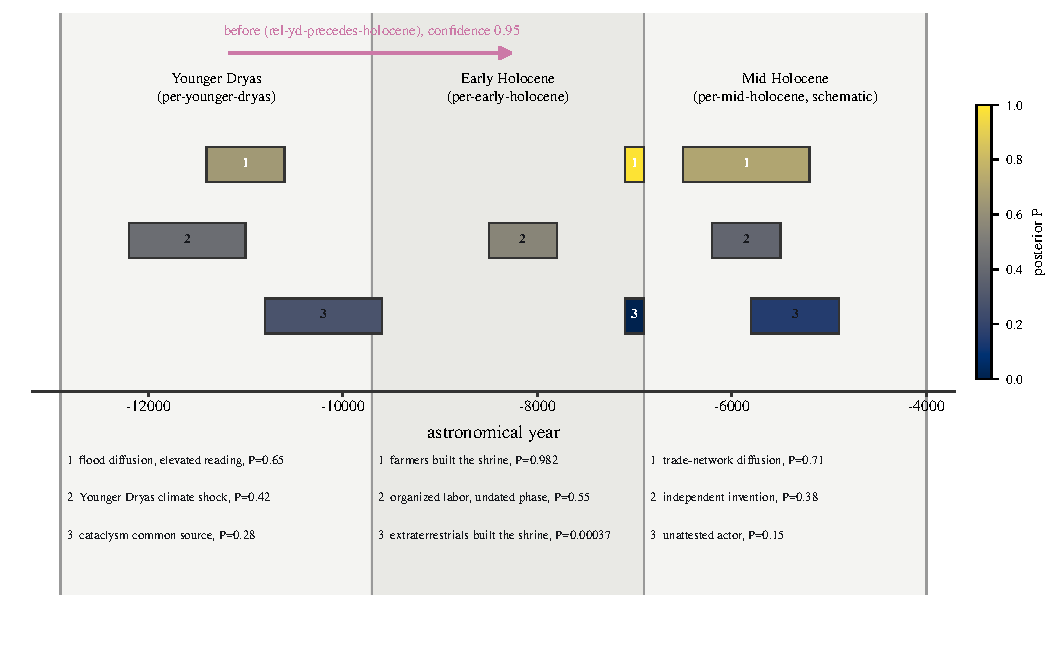
\includegraphics[width=0.76\linewidth]{figures/fig_timeline_view.pdf}
  \caption{A per-bin timeline export across three time bins on the
    astronomical-year axis. Each bin holds its ranked placement
    hypotheses as horizontal bars; bar length is the hypothesis's own
    interval and bar shade is its projected probability $P$. The Younger
    Dryas and Early Holocene bins reuse the exact intervals and $P$ values
    from the cataclysm-diffusion worked example and the Çatalhöyük
    farmers-versus-extraterrestrials opinion of \Cref{sec:belief}; the
    Mid Holocene bin illustrates the same view schematically. The arrow
    spanning the first two bins is a sequence hypothesis carrying its
    Allen relation, \textsc{before} at confidence $0.95$.}
  \label{fig:timeline-view}
\end{figure}

A period's evidence traces back to the \term{retrieval-envelope}{
retrieval envelope} that supplied its dated observation, per
\Cref{sec:engine-loop}: a period's date posterior is only as reliable as
the observations feeding its phase model, and linking each observation to
an immutable envelope means a later re-fetch cannot silently change a
phase model's inputs without a new run id appearing in the model's
provenance.

The engine emits three views over the same scored frontier, none a
verdict: a per-bin view ranking every hypothesis whose \texttt{TIME\_BIN}
falls in that bin, a per-event view collecting every placement sharing an
event's object and place, and a per-pair view collecting every sequence
hypothesis over one ordered pair of events, one entry per Allen relation
the evidence has touched. Display pruning, a top-$N$ cap on a bin, a
collapsed tail on an event, belongs to these views alone; it never
touches what \Cref{sec:combinatorics}'s generator produced.

\section{Combinatorial hypothesis space}
\label{sec:combinatorics}

\Cref{def:placement} and \Cref{def:sequence} fix the two spaces this
engine addresses. With vocabulary sizes a working corpus this size can
reach, $\mathtt{ACTOR} = 40$ (thirty human polities plus ten
concept-ontology actors, including the five non-consensus actors of
\Cref{sec:belief}), $\mathtt{ACTION} = 50$, $\mathtt{OBJECT} = 300$,
$\mathtt{PLACE} = 120$, $\mathtt{TIME\_BIN} = 200$ (century bins across a
20,000-year span), $\mathtt{MECHANISM} = 25$, the two spaces have the
following sizes.

\begin{lemma}[Hypothesis space size]
\label{lem:size}
At the vocabulary sizes stated above,
\begin{equation}
  \label{eq:size-h}
  |H| = 40 \times 50 \times 300 \times 120 \times 200 \times 25 \approx 3.6 \times 10^{11},
\end{equation}
\begin{equation}
  \label{eq:size-hseq}
  |H_{\mathrm{seq}}| = 13 \, |H|^2 \approx 1.7 \times 10^{24}.
\end{equation}
\end{lemma}

\begin{proof}
$|H|$ is the product of the six placement slots' vocabulary sizes by
\Cref{eq:placement-space}; substituting the stated sizes gives
$40 \times 50 = 2{,}000$, $2{,}000 \times 300 = 600{,}000$,
$600{,}000 \times 120 = 72{,}000{,}000$,
$72{,}000{,}000 \times 200 = 14{,}400{,}000{,}000$, and
$14{,}400{,}000{,}000 \times 25 = 3.6 \times 10^{11}$. $|H_{\mathrm{seq}}|$
is the product of $|H|$, the thirteen-value Allen relation vocabulary of
\Cref{def:allen}, and a second copy of $|H|$ by \Cref{eq:sequence-space};
$13 \times (3.6 \times 10^{11})^2 = 13 \times 1.296 \times 10^{23}
\approx 1.7 \times 10^{24}$.
\end{proof}

\Cref{fig:hypothesis-space} plots \Cref{lem:size}'s two sizes,
\Cref{eq:size-h} and \Cref{eq:size-hseq}, alongside a
scale an order of magnitude smaller and one an order of magnitude larger
on every axis, showing how fast the address space grows as a corpus names
more actors, actions, objects, places, time bins, and mechanisms. No
process can materialize a space of $10^{24}$ points; the engine addresses
a point without visiting it.

\begin{figure}[htbp]
  \centering
  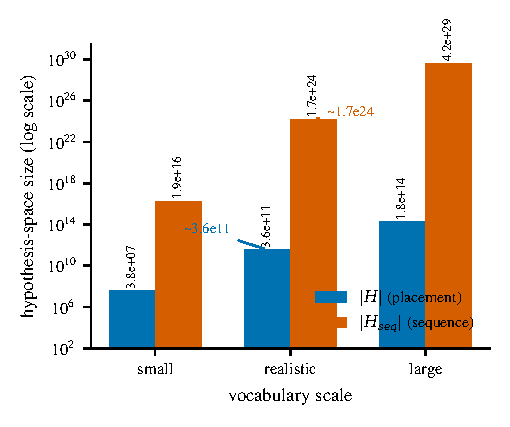
\includegraphics[width=0.60\linewidth]{figures/fig_hypothesis_space.pdf}
  \caption{Placement-space and sequence-space size, $|H|$ and
    $|H_{\mathrm{seq}}|$, at three vocabulary scales on a log axis. The
    realistic scale is \Cref{lem:size}'s own vocabulary sizes; the small
    and large scales hold every axis an order of magnitude below and
    above that scale, showing how fast $|H_{\mathrm{seq}}| = 13|H|^2$
    grows as the corpus names more actors, actions, objects, places,
    time bins, and mechanisms.}
  \label{fig:hypothesis-space}
\end{figure}

\emph{Lazy enumeration.} The generator never iterates $H$ or
$H_{\mathrm{seq}}$. For one evidence cluster, it fixes \texttt{ACTOR},
\texttt{ACTION}, and \texttt{MECHANISM} to their full closed vocabularies,
exotic actors and mechanisms included, evidence or none, and anchors
\texttt{OBJECT}, \texttt{PLACE}, and \texttt{TIME\_BIN} to the values that
cluster names. The product of those six restricted axes, not $H$ itself,
is what one generation pass materializes; the same three anchored axes
stay addressable in full through other passes, an era sweep, an object
sweep, that call \Cref{eq:address} directly on a slot assignment nobody
has iterated to. Scoring and display prune the result; generation does
not, so a hypothesis at near-zero prior still receives an address and a
\term{base-rate}{base rate} the moment it is named.

\begin{lemma}[Address injectivity]
\label{lem:injective}
For a fixed slot order and a fixed vocabulary indexing, $\mathrm{address}$
of \Cref{eq:address} is injective: no two distinct slot assignments share
an address.
\end{lemma}

\begin{proof}
Fix a slot assignment $\mathrm{slots}$ and its address $n =
\prod_k p_k^{v_k+1}$. The primes $p_1, \ldots, p_{13}$ are pairwise
distinct by construction, so $n$'s prime factorization is exactly
$\{p_k^{v_k+1}\}_k$, with no other prime dividing $n$ and no $p_k$
appearing to any other exponent. The fundamental theorem of arithmetic
states this factorization is unique for every positive integer, so
recovering $v_k$ for each $k$, by trial division, dividing by $p_k$ until
it fails and recording the exponent minus one, recovers $\mathrm{slots}$
exactly. Two distinct slot assignments differ in some $v_k$, hence differ
in the exponent of $p_k$ in their respective factorizations, hence
produce distinct $n$.
\end{proof}

\Cref{lem:injective} is why the address needs no lookup table: the
alternative, hashing the slot tuple, is fixed-width and URL-friendly but
opaque, since no hash inversion recovers the slots without a stored
table. The prime encoding recovers them from the integer alone. The
$\mathtt{SHA\text{-}256}$ hash is still stored, as \texttt{address\_hash},
a short display alias the address itself does not need to function.

\begin{definition}[Neighbor mutation]
\label{def:neighbors}
The \term{neighbor-mutation}{neighbor} set of a hypothesis $h$ with slot
assignment $\mathrm{slots}$ is
\begin{equation}
  \label{eq:neighbors}
  N(h) = \bigl\{\, \mathrm{address}(\mathrm{slots}[k \mapsto c]) \;:\;
    k \in \mathrm{slots}, \; c \in \mathrm{vocab}(k), \; c \neq
    \mathrm{slots}[k] \,\bigr\},
\end{equation}
holding every slot but one fixed and ranging that one slot over its
vocabulary. $N(h)$ is the evolver's move set: every one-slot mutation of
$h$, addressed by \Cref{eq:address} without ever materializing $H$ or
$H_{\mathrm{seq}}$ around it.
\end{definition}

\section{Belief model}
\label{sec:belief}

Evidence groups into nine independent modalities: material or
archaeological, textual or documentary, genetic, linguistic, astronomical
or radiometric dating, geological and climate, oral tradition and myth,
iconographic, and model-based inference. For cluster $i$ of kind
$\kappa$, the evidence weight is
\begin{equation}
  \label{eq:cluster-weight}
  s_i = k(\theta_i) \cdot e_i,
\end{equation}
with $k(\theta_i)$ the fixed tier weight of \Cref{def:evidence} and $e_i$
the cluster's edge strength. Where system A's original formula folds
embedding cosine, fuzzy string match, and shared-motif count into one
scalar, $e_i = \min(0.99,\ 0.40 \cos + 0.25\, \mathrm{fuz} + 0.10\,
\mathrm{motif})$, this pass keeps that formula as one named view,
$e_{i,\mathrm{blended\text{-}A}}$, and adds separate views
$e_{i,\mathrm{semantic}}$, $e_{i,\mathrm{lexical}}$, and
$e_{i,\mathrm{motif}}$ for a claim extractor that reports them apart, the
way \texttt{scientific-discovery} keeps task-family, math, operator, and
lexical similarity apart rather than folding structural similarity into
one number. A view-aggregation rule, mean, max, or a learned per-view
weight, is scoped to its own bead and not decided here; every
correlation already scored under the blended formula keeps its stored
confidence unchanged.

Within one \term{evidence-kind}{kind}, corroboration gets diminishing
returns:
\begin{equation}
  \label{eq:diminishing}
  D(n) = 1 + \lambda \ln(1+n), \qquad \lambda = 0.5,
\end{equation}
applied with $n$ replaced by the \term{effective-count}{effective count}
$n_{\mathrm{eff}}$ of \Cref{def:stemma} wherever \Cref{eq:diminishing}
appears, so two texts that copy one archetype count once rather than
twice. Across kinds, let $K_{+}$ (respectively $K_{-}$) be the number of
distinct kinds carrying supporting (refuting) evidence, grouped into three
families, material trace, textual trace, and inference, with
$\mathrm{kind\_distance}$ equal to $1$ across families and $0$ within
one. The cross-kind independence bonus is
\begin{equation}
  \label{eq:cross-kind}
  X(K) = 1 + 0.3 \sum_{\mathrm{pairs}} \mathrm{kind\_distance}(\mathrm{pair}),
\end{equation}
rewarding corroboration from two different kinds over two clusters of one
kind. The pooled supporting and refuting weights are
$S_{+} = X(K_{+}) \sum_{\kappa} D(n_{\mathrm{eff},\kappa}) \sum_{i \in
\kappa} s_i$ and $S_{-}$ symmetrically for refuting evidence, with each
$s_i$ the per-cluster evidence weight of \Cref{eq:cluster-weight}.

\begin{definition}[Opinion from evidence sums]
\label{def:opinion-fusion}
Fix the total-ignorance weight $W = 2$. Given pooled supporting and
refuting weights $S_{+}$ and $S_{-}$ for a hypothesis $h$, let
$r = S_{+}$ and $s = S_{-}$ (each already carrying its own
\Cref{eq:diminishing} discount). The fused opinion is
\begin{equation}
  \label{eq:opinion-sum}
  b(h) = \frac{r}{r+s+W}, \qquad
  d(h) = \frac{s}{r+s+W}, \qquad
  u(h) = \frac{W}{r+s+W}, \qquad
  a(h) = \operatorname{sigmoid}\bigl(L_{\mathrm{prior}}(h)\bigr),
\end{equation}
where $L_{\mathrm{prior}}(h) = \sum_{\mathrm{slots}} \ell(c)$ sums the
\term{prior-logit}{prior logit} of every slot's concept, per
\Cref{def:slot}. Lean counterpart: \texttt{Bucket.Belief.fromEvidence},
proved over its \texttt{Rat} counterpart \texttt{fromEvidenceQ}
(\Cref{lem:opinion-sum}).
\end{definition}

\begin{lemma}[Normalization and probability bound]
\label{lem:opinion-sum}
For every hypothesis $h$ scored by \Cref{eq:opinion-sum},
$b(h) + d(h) + u(h) = 1$ and $P(h) \in [0,1]$.
\end{lemma}

\begin{proof}
By \Cref{eq:opinion-sum}, $b(h) + d(h) + u(h) = \frac{r+s+W}{r+s+W} = 1$
whenever $r, s \geq 0$ and $W > 0$, both guaranteed by construction
($S_{+}, S_{-} \geq 0$ as sums of nonnegative tier weights, and $W = 2$
fixed). For the bound, $P(h) = b(h) + a(h) u(h)$ by \Cref{eq:projection}.
Since $a(h) = \operatorname{sigmoid}(\cdot) \in [0,1]$ and $u(h) \in
[0,1]$ by the normalization just shown, $a(h) u(h) \in [0, u(h)]$, so
$P(h) \in [b(h), b(h) + u(h)]$. Since $b(h) + u(h) \leq b(h) + d(h) +
u(h) = 1$ and $b(h) \geq 0$, both endpoints lie in $[0,1]$, hence
$P(h) \in [0,1]$.
\end{proof}

At zero evidence, $r = s = 0$, so $b = d = 0$ and $u = 1$ by
\Cref{eq:opinion-sum}, giving $P(h) = a(h)$ exactly (Lean:
\texttt{Bucket.Belief.u\_eq\_one\_of\_no\_evidence}): a hypothesis nobody
has examined reads at its prior, with a stated uncertainty mass of $1$,
rather than at an unmarked point estimate indistinguishable from a
refuted one. Ranking stays compatible with the corpus's existing
log-odds signal: with $\Theta_{\mathrm{temporal}}(h)$ the agreement
between $h$'s stated interval and its period's date posterior (zero when
no date claim is tested), the ranking score
\begin{equation}
  \label{eq:rank}
  L(h) = \ln\!\left(\frac{P(h)}{1-P(h)}\right) + \Theta_{\mathrm{temporal}}(h)
\end{equation}
is a read-out of the opinion rather than the primitive it is built from,
so the tournament of \Cref{sec:engine-loop} keeps working on it
unmodified.

\emph{Contradiction falls out on its own.} The corpus's original
truth-score formula subtracted a separate contradiction penalty
$\Omega_{\mathrm{contradiction}} = \mu \cdot \min(D(n_{+}) S_{+},
D(n_{-}) S_{-})$, with $\mu = 0.5$, whenever both sides carried real
weight. \Cref{eq:opinion-sum} needs no such term: when $b(h)$ and $d(h)$
sit close together, $P(h)$ sits close to $a(h)$, since $b = d$ gives
$P = (1-u)/2 + a u$, which reduces to $a$ as $u \to 1$ and to $1/2$ only
when $a = 1/2$. A contested hypothesis settles at the prior it carries
instead of landing at even odds by default, so $\mu$ has no counterpart
in \Cref{eq:opinion-sum} or \Cref{eq:rank}: the opinion model absorbs
what $\Omega_{\mathrm{contradiction}}$ did.

\Cref{fig:opinion-triangle} plots the opinion triangle, and
\Cref{fig:evidence-accumulation} plots $b$, $d$, $u$, and $P$ against a
growing evidence count under \Cref{eq:opinion-sum} and
\Cref{eq:diminishing}, for a fixed tier weight and an uninformative base
rate $a = 0.5$: panel (a) accumulates supporting evidence only, panel (b)
mixes support and refutation at a $2$-to-$1$ ratio, and both panels show
$u$ shrinking as $r+s$ grows regardless of which side leads.

\begin{figure}[htbp]
  \centering
  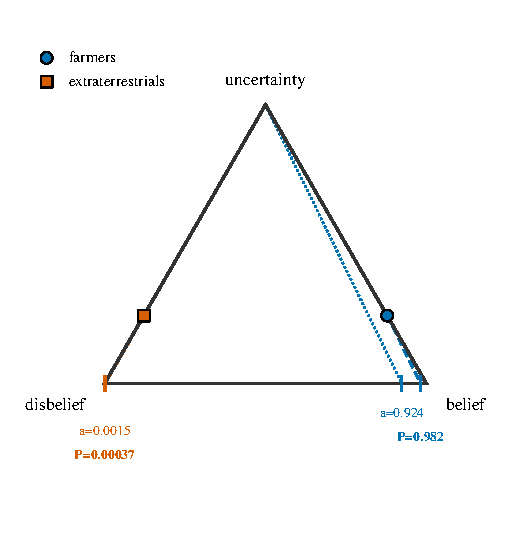
\includegraphics[width=0.54\linewidth]{figures/fig_opinion_triangle.pdf}
  \caption{The subjective-logic opinion triangle, vertices belief,
    disbelief, and uncertainty, with the Çatalhöyük worked example of
    \Cref{tab:worked-example}. Each opinion $(b,d,u)$ plots at its
    barycentric position; the projected probability $P = b + au$ for a
    base rate $a$ reads off the base edge along the line through the
    opinion point running parallel to the segment from the uncertainty
    vertex to the base-rate point $(a, 0)$ on that edge.}
  \label{fig:opinion-triangle}
\end{figure}

\begin{figure}[htbp]
  \centering
  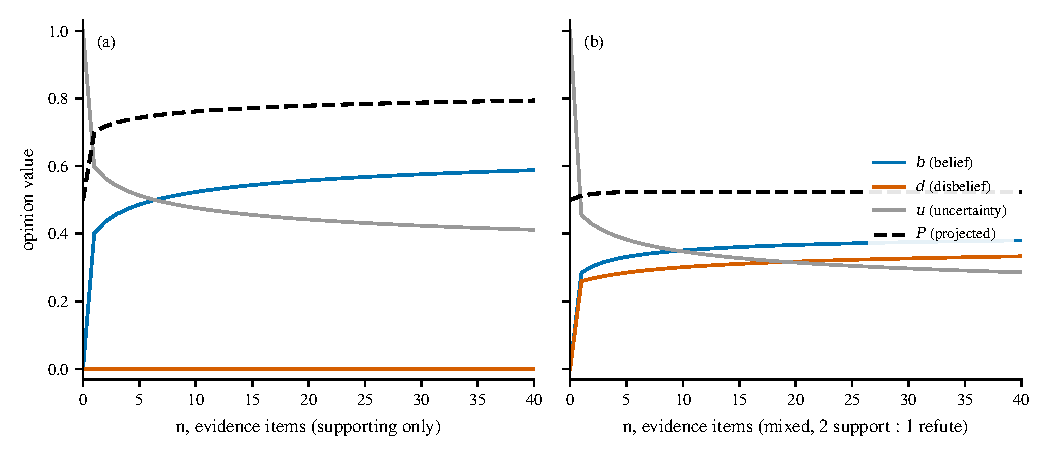
\includegraphics[width=0.78\linewidth]{figures/fig_evidence_accumulation.pdf}
  \caption{Belief, disbelief, uncertainty, and projected probability
    against the number of independent evidence items $n$, for one
    hypothesis at a fixed tier weight and an uninformative base rate
    $a = 0.5$. Panel (a) accumulates supporting evidence only; panel (b)
    mixes support and refutation at a $2$-to-$1$ ratio. Both panels use
    \Cref{eq:opinion-sum} with $W=2$ and the diminishing-returns discount
    of \Cref{eq:diminishing} applied to each side before it enters $r$
    and $s$.}
  \label{fig:evidence-accumulation}
\end{figure}

\emph{Detectability as a likelihood ratio.} An absence of evidence is
data only when evidence would likely have survived and been found.
Detectability (\Cref{def:detect}) scales absence evidence in place of a
flat tier:
\begin{equation}
  \label{eq:detectability}
  e_{\mathrm{absence}} = \delta(\mathrm{period}, \mathrm{medium},
    \mathrm{region}) \cdot e_{\mathrm{raw\text{-}absence}},
\end{equation}
read as the likelihood ratio between observing no evidence when $h$ is
true and observing no evidence when $h$ is false: as $\delta \to 0$ that
ratio approaches $1$ and absence stops discriminating; as $\delta \to 1$
it recovers the flat-tier treatment as its high-detectability limit. A
positive find in a low-$\delta$ context is the rarer event under this
same ratio, so a reviewer can weight it up by the same $\delta$ on the
corroboration side, by hand rather than by a default rule.

\emph{Worked example.} Fix \texttt{ACTION} = built, \texttt{OBJECT} =
Çatalhöyük shrine, \texttt{PLACE} = Çatalhöyük, \texttt{TIME\_BIN} =
$-7000$-century, and vary \texttt{ACTOR} and \texttt{MECHANISM}.
\texttt{neolithic-farmers-anatolia} (prior logit $2.0$) paired with
\texttt{organized-human-labor} ($0.5$) gives $L_{\mathrm{prior}} = 2.5$;
\texttt{extraterrestrials} ($-4.0$) paired with \texttt{unknown-
technology} ($-2.5$) gives $L_{\mathrm{prior}} = -6.5$. Both hypotheses
already carry an address and a base rate before either is read against a
source. Pool three evidence items against both, flipped by which
\texttt{ACTOR} they favor: a radiocarbon-dated construction fill with
hand-tool marks (material, T1, $e = 0.9$), a tool-mark microwear study
(material, T2, $e = 0.5$), and the documentary silence across every
tradition on a non-human builder at the site (textual, T3, $e = 0.6$).
All three support farmers and refute the extraterrestrial reading. Within
the material kind,
\begin{equation}
  \label{eq:material-kind}
  \sum k \cdot e = 2.0(0.9) + 1.5(0.5) = 2.55, \quad n_{\mathrm{eff}}=2,
  \quad D(2) = 1.549 \;\Rightarrow\; 3.951,
\end{equation}
and within the textual kind,
\begin{equation}
  \label{eq:textual-kind}
  \sum k \cdot e = 1.0(0.6) = 0.60, \quad n_{\mathrm{eff}}=1,
  \quad D(1) = 1.347 \;\Rightarrow\; 0.808.
\end{equation}
The pooled weight is $E = 4.759$ across $K=2$ kinds spanning one
cross-family pair, so $X(2) = 1 + 0.3(1) = 1.3$ by \Cref{eq:cross-kind}
and $S_{+} = 1.3 \times 4.759 = 6.186$ for the farmers reading,
$S_{-} = 6.186$ for the extraterrestrial reading. \Cref{tab:worked-example}
carries both readings through \Cref{eq:opinion-sum}.

\begin{table}[htbp]
  \centering
  \caption{Çatalhöyük shrine-construction worked example: the base rate
    before any evidence is pooled, and the opinion after pooling the
    three items of \Cref{eq:material-kind} and \Cref{eq:textual-kind}.}
  \label{tab:worked-example}
  \begin{tabular}{@{}lcc@{}}
    \toprule
    Quantity & Farmers reading & Extraterrestrial reading \\
    \midrule
    $L_{\mathrm{prior}}$        & $2.5$    & $-6.5$    \\
    $a = \operatorname{sigmoid}(L_{\mathrm{prior}})$ & $0.924$  & $0.0015$  \\
    $r$ (pooled support)        & $6.186$  & $0$       \\
    $s$ (pooled refutation)     & $0$      & $6.186$   \\
    $b$                          & $0.756$  & $0.000$   \\
    $d$                          & $0.000$  & $0.756$   \\
    $u$                          & $0.244$  & $0.244$   \\
    $P = b + a u$                & $0.982$  & $0.00037$ \\
    \bottomrule
  \end{tabular}
\end{table}

Both readings land the same direction as the corpus's original sigmoid
posterior ($\tau \approx 0.9998$ and $\tau \approx 0.0000031$ under
\Cref{eq:rank} without the opinion layer) and stay separated, but land
less extreme on each side: the opinion form keeps $24$ percent of the
pool as stated uncertainty, so the same three findings move the
mainstream reading to $98$ percent instead of four nines, and the exotic
reading to four parts in ten thousand instead of three parts in a
million. The evidence pooled is unchanged; what changed is that the model
now states how much of its confidence rests on the prior against how much
rests on what was found.

\section{Structural unknowns}
\label{sec:unknowns}

A gap node (\Cref{def:gap}) names an unexcavated site, an untranslated
text, an undated stratum, or an unread archive, and the hypotheses reading
it would move. Its ranking score folds five factors, borrowed from
\texttt{scientific-discovery}'s active-retrieval priority rather than
resting on expected uncertainty reduction alone:
\begin{equation}
  \label{eq:voi}
  \mathrm{voi}(\mathrm{gap}) = w_1 \, \Delta u_{\mathrm{expected}}
    + w_2 \, \mathrm{novelty}(\mathrm{gap})
    + w_3 \, \mathrm{coverage\_gap}(\mathrm{period})
    + w_4 \, \mathrm{historical\_gap}(\mathrm{period})
    + w_5 \, \mathrm{disagreement}(\mathrm{gap}),
\end{equation}
with weights $w_1, \ldots, w_5$ starting uniform and calibrated against
the holdout runs of \Cref{sec:calibration}. Since new evidence always
adds to $r$ or $s$ and shrinks $u$ by \Cref{eq:opinion-sum}, $\Delta
u_{\mathrm{expected}}$ is well defined for every gap without running the
retrieval it names; the active-learning queue \Cref{eq:voi}'s score
orders is the mirror of \Cref{sec:calibration}'s founder-review queue,
one ranks what to judge, the other ranks what to go look at next.

Every slot's vocabulary (\Cref{def:slot}) carries a reserved
\term{other-slot}{\texttt{OTHER}} concept with a Dirichlet-process
new-concept probability
\begin{equation}
  \label{eq:new-concept}
  P(\mathrm{new\ concept\ in\ slot}) = \frac{\alpha}{\alpha + N}
\end{equation}
\autocite{ferguson1973bayesian}, with $N$ the count of concept instances
seen so far in that slot and $\alpha$ a per-slot concentration constant. A
hypothesis naming \texttt{ACTOR: other-unnamed} still receives an address
by \Cref{eq:address} and a base rate by \Cref{eq:opinion-sum}.

Missing mass (\Cref{def:missingmass}) is estimated by running generation
several times under different explore-or-exploit seeds or prior profiles
and treating each run's frontier as a sample: $f_1/N$ estimates the
unseen share, and the Chao1 richness estimate
\begin{equation}
  \label{eq:chao1}
  S_{\mathrm{est}} = S_{\mathrm{obs}} + \frac{f_1^2}{2 f_2}
\end{equation}
\autocite{colwell1994estimating,chao1987estimating} sizes the total
address space reachable from the evidence on file. The same
estimator applies to evidence discovery per period, counting discovery
events instead of hypotheses. \Cref{fig:missing-mass} shows both
quantities against a growing number of generation runs, for a simulated
generator drawing from a Zipf-distributed pool of $5{,}000$ addressable
hypotheses: the Chao1 curve's gap below the pool's known true size after
60 runs of 40 draws each is the caution against reporting a coverage
number before the estimator has had enough runs to converge on it.

\begin{figure}[htbp]
  \centering
  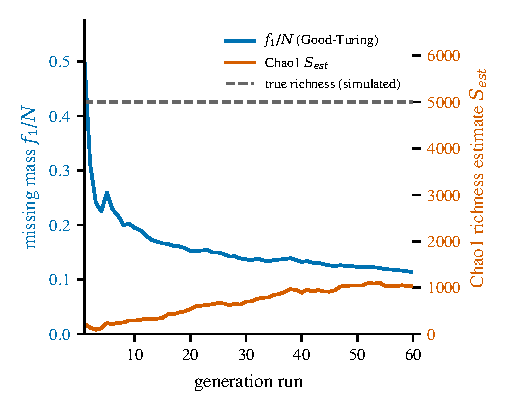
\includegraphics[width=0.64\linewidth]{figures/fig_missing_mass.pdf}
  \caption{Good-Turing missing mass $f_1/N$ against the number of
    generation runs, with the Chao1 richness estimate of
    \Cref{eq:chao1} on a second axis, for a simulated generator drawing
    from a Zipf-distributed pool of $5{,}000$ addressable hypotheses. The
    dashed line marks the pool's known true size; the Chao1 curve's gap
    below that line after 60 runs of 40 draws each is the same caution
    \Cref{sec:calibration} raises against reporting a coverage number
    before an estimator has converged.}
  \label{fig:missing-mass}
\end{figure}

\term{coverage-share}{Coverage share} replaces the claim that generation
produces the full set. For each time bin,
\begin{equation}
  \label{eq:coverage}
  \mathrm{coverage\_share}(\mathrm{bin}) =
    \frac{\mathrm{hypotheses\_generated\_and\_scored}(\mathrm{bin})}
    {S_{\mathrm{est}}(\mathrm{bin})},
\end{equation}
reported as an interval, $\mathrm{ci\_low}$ and $\mathrm{ci\_high}$, since
Chao1 carries an analytic variance. A bin's interval is reported only
after it passes a three-part audited-saturation gate, borrowed from
\texttt{scientific-discovery}: a minimum iteration count, recent
normalized novelty below threshold, and stable coverage strata across
period, tradition, evidence kind, and rights tier. A bin that has not
passed the gate reports a status of generating in place of an interval,
so an early, narrow-looking, and misleadingly confident interval never
appears before the search has run long enough to earn one.

\Cref{fig:detectability} shows one slice of the per-period,
per-medium, per-region detectability table \Cref{eq:detectability}
scales absence evidence by: rows run from the Upper Paleolithic through
the Iron Age and Classical period, columns are the nine evidence kinds of
\Cref{sec:belief}, and the illustrated values show textual detectability
near zero before writing, rising once a period has a literate record,
while genetic detectability rises toward the present.

\begin{figure}[htbp]
  \centering
  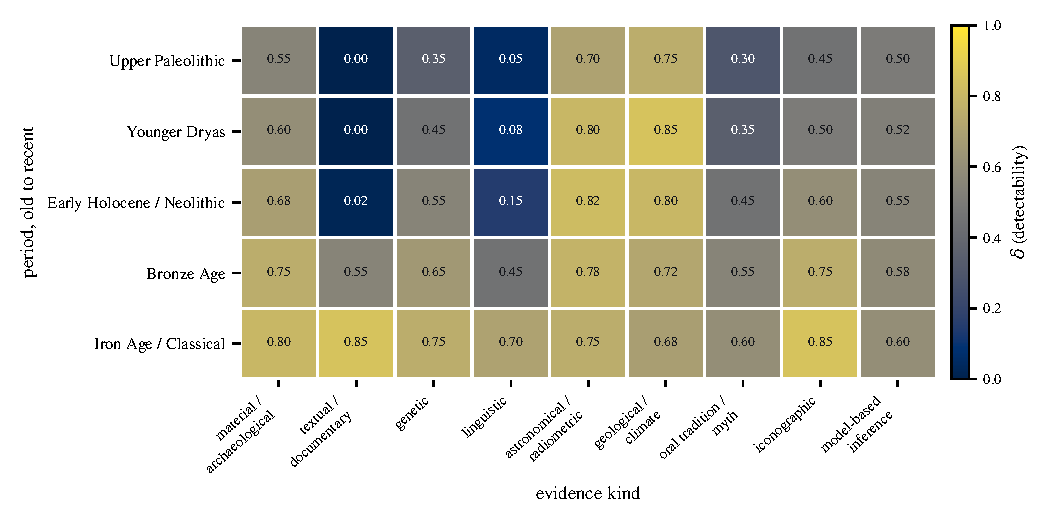
\includegraphics[width=0.76\linewidth]{figures/fig_detectability.pdf}
  \caption{A toy detectability table $\delta(\mathrm{period},
    \mathrm{evidence\ kind})$, one slice of the per-period, per-medium,
    per-region table of \Cref{def:detect}. Rows run from the Upper
    Paleolithic to the Iron Age and Classical period; columns are the
    nine evidence kinds of \Cref{sec:belief}. Values are illustrative:
    textual detectability sits near zero before writing and rises once a
    period has a literate record, while genetic detectability rises
    toward the present.}
  \label{fig:detectability}
\end{figure}

A \term{surprise-event}{surprise event} is logged when new evidence
matches no hypothesis address at any slot-value combination the generator
has materialized. Its rate, events per period divided by total evidence
discovered that period, is a health metric read two ways: a rising rate
says the ontology trails the evidence, a falling rate says either
convergence or a generator that has stopped looking, and the two readings
are told apart by whether evidence volume that period held steady.

\term{prior-profile-robustness}{Prior-profile robustness} scores one
hypothesis under four prior profiles, consensus ($L_{\mathrm{prior}}$ as
computed today), skeptic (flat or negative priors on every non-attested
extraordinary claim), fringe (elevated priors on the exotic actors and
mechanisms of \Cref{sec:belief}), and uniform ($L_{\mathrm{prior}} = 0$
everywhere):
\begin{equation}
  \label{eq:robustness}
  \mathrm{robustness}(h) = 1 - \Bigl(\max_p P_p(h) - \min_p P_p(h)\Bigr),
\end{equation}
where $P_p(h)$ recomputes \Cref{eq:opinion-sum} and
\Cref{eq:projection} with $a(h)$ read from profile $p$'s
$L_{\mathrm{prior}}$. A hypothesis with high $\mathrm{robustness}(h)$
earns more trust than one whose rank flips depending on which profile
scores it.

\section{Engine loop}
\label{sec:engine-loop}

\Cref{fig:architecture} lays out the full loop this engine runs, generate,
critique, rank, evolve, review, the shape DeepMind's AI co-scientist runs
over biomedical literature \autocite{gottweis2025coscientist}, with
MC-NEST's explicit explore-or-exploit control on the ranking step
\autocite{rabby2024mcnest}.

\begin{figure}[htbp]
  \centering
  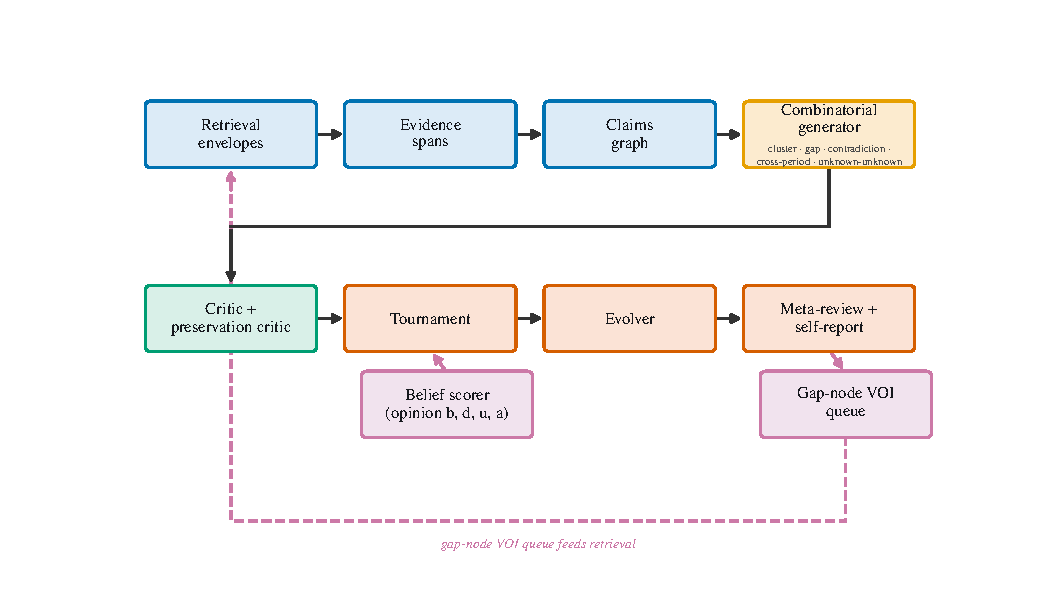
\includegraphics[width=0.80\linewidth]{figures/fig_architecture.pdf}
  \caption{The hypothesis engine's generation loop. Retrieval envelopes
    ground evidence spans, which populate the claims graph; the
    combinatorial generator draws placement and sequence hypotheses
    through four generator kinds, cluster, gap, contradiction, and
    cross-period, plus the unknown-unknown generator, which proposes slot
    values outside the current vocabulary. Surviving hypotheses pass
    through the critic and preservation critic, a belief scorer feeds the
    ranking tournament, and the evolver recombines, splits, and
    generalizes the frontier before meta-review and self-report close the
    run. The gap-node value-of-information queue reads the self-report
    and routes back into retrieval.}
  \label{fig:architecture}
\end{figure}

\emph{Generator.} Four generator kinds feed the frontier: evidence
clusters, grouped by embedding, fuzzy match, and shared-motif similarity,
enumerate a placement or sequence per \Cref{eq:placement-space} or
\Cref{eq:sequence-space}; claim gaps yield a hypothesis proposing a
missing predicate on an under-specified node; contradictions between two
comparable-prior claims yield a hypothesis reconciling or arbitrating
them; cross-period analogies over a recurring motif yield a hypothesis
testing common cause against independent recurrence. A fifth role, the
unknown-unknown generator, proposes only slot values outside the current
vocabulary, feeding the open-world mass of \Cref{eq:new-concept}
directly; it never scores, only proposes. Every hypothesis this stage
produces receives an address by \Cref{eq:address} before scoring, per
\Cref{sec:combinatorics}'s lazy-enumeration rule.

\emph{Critic and preservation critic.} A rule-and-model pass rejects
combinations the claims graph itself contradicts, an actor not attested
inside the proposed time bin, a place outside every tradition the actor
belongs to, before scoring runs. The preservation critic asks, for every
surviving hypothesis, what evidence would exist if it were true and
whether that evidence could have survived to be found, reading
\Cref{def:detect}'s table before recommending rejection, so a low
detectability score explains an absence before falsity does.

\emph{Ranking tournament.} Elo is seeded from the posterior,
$\mathrm{Elo}_0 = 1500 + 400 \operatorname{logit}(P(h))$, then updated by
pairwise debate rounds. Every fixed number of rounds, \Cref{eq:opinion-sum}
recomputes exactly and Elo reseeds from it, keeping the projected
probability authoritative over the tournament's running score rather than
the reverse.

\emph{Evolver.} \Cref{def:neighbors}'s one-slot mutation
(\Cref{eq:neighbors}) is the evolver's smallest move; it also recombines
two hypotheses sharing a cluster into
one with a merged claim set, splits an overbroad hypothesis into narrower
dated children, and generalizes a set of narrow siblings that agree into
one broader periodization claim.

\emph{Self-report and target-blind generation.} Every run emits a
\term{self-report}{self-report}: its assumptions, which slot vocabularies
it judged incomplete, its missing-mass estimate (\Cref{eq:chao1}), and its
calibration score against the holdout tests of \Cref{sec:calibration}.
\texttt{scientific-discovery}'s charter states that its retrieval never
biases corpus construction toward quantum relevance; this engine
generalizes that rule as \term{target-blind}{target-blind generation}:
generation stays complete and scored the same way regardless of which
target reading, orthodox, fringe, or any consensus status between, a
hypothesis would end up supporting. A per-run self-report line states
whether the generator's proposal rate for non-consensus actor or
mechanism values held steady against the run before it; a falling rate
under stable evidence volume is the same health signal
\Cref{sec:unknowns}'s surprise-rate tracks, read here for target-blindness
instead of vocabulary drift. The model's own trained-in sense of a
period, cited in \Cref{sec:related} as Hist-LLM's near-46-percent recall
against Seshat's coded judgments, enters as one evidence kind,
\texttt{model-prior}, at a low tier, with its own reliability tracked run
over run; it never counts as truth on its own.

\emph{Target-blind corpus construction and retrieval provenance.} Every
fetch a mirror job makes is written as an immutable
\term{retrieval-envelope}{retrieval envelope}, linked to a
\texttt{RetrievalRun} id, so a later re-fetch cannot silently change what
an earlier run found. Once a fetch routes through the
\texttt{x402-research-gateway}, the envelope carries the gateway's
manifest fingerprint, protocol version, and citation and lineage counts;
until that path exists for history sources, the envelope still carries
the provenance shape against the existing corpus mirror job, so the
provenance layer needs no rework when the gateway path lands.

\section{Calibration and pilot design}
\label{sec:calibration}

Two holdout splits test whether a posterior predicts unseen evidence, run
inside a named campaign rather than an ad hoc script call, borrowing
\texttt{scientific-discovery}'s discipline of a frozen work set sampled
across explicit strata (period, tradition, evidence kind, rights tier)
before generation starts, with extraction, scoring, and matching failures
recorded in the campaign's run log before any repair lands.

\emph{Discovery-date holdout.} Split each claim's evidence at a cutoff on
its recorded discovery date, recompute \Cref{eq:opinion-sum} from
pre-cutoff evidence only, then check whether the post-cutoff evidence's
support sign matches what the pre-cutoff opinion implied. Score the match
rate as a Brier score across every hypothesis with holdout evidence. The
first campaign runs this split on a well-dated modern timeline, chosen
because its ground truth is settled well enough that a wrong prediction
is attributable to the model rather than to the timeline's own
uncertainty.

\emph{Period holdout.} Withhold every claim assigned to one period,
generate hypotheses from the remaining periods only, then test the
withheld period's real claims against the predicted slot tuples for a
match rate. This checks the engine against the claims graph for that
period rather than against a trained model's memorized sense of it, the
caution the Hist-LLM benchmark raises about a model's memorized sense of
a period from training data (\Cref{sec:related}).

Both Brier scores feed a recalibration pass over the tunable constants
$\lambda$ (\Cref{eq:diminishing}) and $W$ (\Cref{eq:opinion-sum}), fit by
grid search and re-run on a schedule as the corpus grows. The corpus's
original contradiction penalty $\mu$ takes no recalibration pass of its
own: \Cref{sec:belief} folds contradiction into the opinion model
directly rather than carrying $\mu$ forward as a separate term. Each
recalibration carries a run id, the same audit pattern the corpus's
mirror jobs already write.

Once the discovery-date holdout has run on a well-dated timeline, the
period holdout runs as a frozen campaign against a contested period,
chosen from the two candidates in \Cref{tab:pilot-periods}. Neither
candidate has been run; the table states what each would exercise, not
what either would show.

\begin{table}[htbp]
  \centering
  \caption{Two candidate periods for the first frozen period-holdout
    campaign, stated as design options. Neither has been run; no result
    is claimed for either.}
  \label{tab:pilot-periods}
  \begin{tabular}{@{}p{3.3cm}p{2.6cm}p{7.5cm}@{}}
    \toprule
    Period & Date range & Evidence kinds exercised \\
    \midrule
    Younger Dryas boundary & 12.9 to 11.7 ka &
      Astronomical and radiometric dating, geological and climate,
      material and archaeological (impact-proxy strata), oral tradition
      and myth (flood-motif correlations already on file). Detectability
      is low across every kind, a preliterate period with a thin,
      contested stratigraphic record. \\
    \addlinespace
    Neolithic Anatolia & 9500 to 7000 BCE &
      Material and archaeological (Çatalhöyük and comparable sites),
      genetic (ancient-DNA population continuity), linguistic
      (proto-language dispersal claims), model-based inference. This
      paper's own worked example (\Cref{tab:worked-example}) sits inside
      this window. \\
    \bottomrule
  \end{tabular}
\end{table}

\section{Limitations}
\label{sec:limitations}

This is a design paper: every claim above is a derivation, checked in
\Cref{sec:combinatorics} and \Cref{sec:belief} and pointed at its Lean
listing in \Cref{app:lean}, and no empirical result is claimed anywhere in
it. Several limitations follow directly from that scope.

The model-prior evidence kind (\Cref{sec:engine-loop}) mitigates the
generating model's own trained-in sense of a period only in part: it
lowers that sense to a low-tier, tracked-reliability kind rather than an
unaccounted background assumption, but it does not remove the sense
itself, and a model whose training corpus underrepresents a tradition
still generates fewer hypotheses favoring that tradition's reading before
any evidence is read.

The constants $W = 2$ (\Cref{eq:opinion-sum}) and $\lambda = 0.5$
(\Cref{eq:diminishing}) are uncalibrated: they are the values the
corpus's existing truth-score formula already used, kept fixed through
the move to an opinion model rather than refit to it.
\Cref{sec:calibration}'s recalibration pass is designed but has not run.

The reserved \term{other-slot}{\texttt{OTHER}} concept
(\Cref{eq:new-concept}) gives a value outside the closed vocabulary an
address and a share of the probability mass, without naming that value:
a hypothesis routed through \texttt{OTHER} carries a base rate and a
place in the frontier, leaving the specific actor, action, or mechanism
a reader would need to go test it unnamed. Every slot's vocabulary stays
closed at the concept level even though its reserved mass is open;
naming what \texttt{OTHER} stands for on a given run stays a curation
step outside \Cref{eq:new-concept} itself.

Detectability (\Cref{def:detect}) and gap nodes (\Cref{def:gap}) have no
Lean counterpart in this pass; \Cref{app:lean} names both as pending
rather than proving a stand-in for either. The detectability table itself
is stated as illustrative in \Cref{fig:detectability}: its real values
are a claim about the corpus, one new excavation or archive access can
revise.

Two gaps sit inside the Lean listings themselves (\Cref{app:lean}).
First, \texttt{Bucket.Belief.Opinion} is the \texttt{Float} shape the
running system computes with, and every proved claim, \Cref{lem:opinion-sum}
included, is proved instead over \texttt{Bucket.Belief.OpinionQ}'s
\texttt{Rat} counterpart, since \texttt{Float} carries no Lean order
structure a proof can use; nothing in this pass bounds how far a running
\texttt{Float} computation can drift from its \texttt{Rat} proof. Second,
\texttt{Bucket.Address.encode\_injective}, the Lean statement of
\Cref{lem:injective}'s general injectivity claim, is left \texttt{sorry}:
the pen-and-paper proof in \Cref{sec:combinatorics} stands on the
fundamental theorem of arithmetic, and mechanizing that argument for an
arbitrary vocabulary size needs Mathlib's \texttt{Nat.factorization} or
an equivalent unique-factorization development, unavailable in this
Mathlib-free build. Only the bounded case,
\texttt{encode\_injective\_bounded}, is proved in full, by exhaustive
computation over tuples with every slot index below $2$.

The Younger Dryas and Neolithic Anatolia candidates of
\Cref{tab:pilot-periods} are both contested periods by design, chosen to
exercise different evidence-kind mixes; neither is a validation set with
an agreed ground truth, so the period holdout's match rate on either
reads against the claims graph on file alone. A campaign run on one
candidate does not transfer its calibration to the other without its own
holdout pass.

Prior-profile robustness (\Cref{eq:robustness}) reports a spread across
four named profiles chosen by hand; it is not a claim that these four
span every reasonable prior an outside reviewer might hold, only that a
hypothesis stable across these four has cleared one check a hypothesis
stable across zero has not.

\printbibliography

\appendix
\small

\section{Lean listings}
\label{app:lean}

Every definition in \Cref{sec:prelim} names a Lean counterpart under
\texttt{lean/Bucket/}, a minimal Lake project (\texttt{lean-toolchain}
pinned to \texttt{leanprover/lean4:v4.33.1}, one \texttt{lean\_lib}
target) built by \texttt{make lean}, mirroring
\texttt{papers/template/lean/}. All six files below are on disk and
\texttt{lake build} passes over every one of them; the guard on each
listing below is a defensive fallback rather than a live condition.

\paragraph{Bucket.Timeline} (\Cref{def:interval}, \Cref{def:allen}).
\bucketlean{lean-snapshots/Timeline.lean}{lean/Bucket/Timeline.lean}{Bucket.Timeline.Interval, Bucket.Timeline.AllenRelation}

\paragraph{Bucket.Concept} (\Cref{def:slot}).
\bucketlean{lean-snapshots/Concept.lean}{lean/Bucket/Concept.lean}{Bucket.Concept.Slot}

\paragraph{Bucket.Hypothesis} (\Cref{def:placement}, \Cref{def:sequence}).
\bucketlean{lean-snapshots/Hypothesis.lean}{lean/Bucket/Hypothesis.lean}{Bucket.Hypothesis.Placement, Bucket.Hypothesis.Sequence}

\paragraph{Bucket.Address} (\Cref{def:address}, \Cref{lem:injective}).
\bucketlean{lean-snapshots/Address.lean}{lean/Bucket/Address.lean}{Bucket.Address.encode}

\paragraph{Bucket.Belief} (\Cref{def:opinion}, \Cref{def:projection},
\Cref{def:opinion-fusion}, \Cref{lem:opinion-sum}).
\bucketlean{lean-snapshots/Belief.lean}{lean/Bucket/Belief.lean}{Bucket.Belief.Opinion, Bucket.Belief.fromEvidence, Bucket.Belief.project}

\paragraph{Bucket.Unknowns} (\Cref{def:missingmass}).
\bucketlean{lean-snapshots/Unknowns.lean}{lean/Bucket/Unknowns.lean}{Bucket.Unknowns.missingMass}

\texttt{Bucket.Address.encode\_injective}, the Lean statement of
\Cref{lem:injective}'s general injectivity claim, is the one result this
paper needs machine-checked and leaves \texttt{sorry}, per
\Cref{sec:limitations}; \texttt{Bucket.Belief} discharges
\Cref{lem:opinion-sum} in full, as \texttt{sum\_eq\_one} and
\texttt{project\_mem\_unit} over the \texttt{Rat}-typed
\texttt{fromEvidenceQ}, and \texttt{Bucket.Timeline} discharges seven
further theorems characterizing \texttt{relate}, none of them stated as
a lemma in the body. \Cref{def:stemma}'s effective count and
\Cref{def:detect}'s detectability and \Cref{def:gap}'s gap nodes carry
no listing here, per \Cref{sec:limitations}.

The verbatim block below is \texttt{lake build}'s own output for this
project, run from \texttt{lean/} with \texttt{PATH} carrying
\texttt{\textasciitilde/.elan/bin} (Lean 4.33.1, Lake 5.0.0), captured
for this pass. Lake marks each job with a Unicode check mark or warning
triangle; this build has no Unicode math font either (the same gap
\texttt{make\_lean\_snapshots.py}'s header documents), so those two
glyphs are transliterated to \texttt{OK} and \texttt{WARN} below and
nothing else in the line is altered:

% voice-ignore-next 10
\begin{verbatim}
OK [2/9] Built Bucket.Concept (297ms)
OK [3/9] Built Bucket.Belief (354ms)
OK [4/9] Built Bucket.Unknowns (314ms)
WARN [5/9] Built Bucket.Address (1.7s)
warning: Bucket/Address.lean:57:8: declaration uses `sorry`
OK [6/9] Built Bucket.Timeline (12s)
OK [7/9] Built Bucket.Hypothesis (223ms)
OK [8/9] Built Bucket (150ms)
Build completed successfully (9 jobs).
\end{verbatim}

The one warning is \Cref{lem:injective}'s open item: every other module
builds with no warning.

\section{Bead list}
\label{app:beads}

\texttt{CROSSWALK-QUANTUM-ALGORITHM-DISCOVERY.md} \S5 re-cuts every bead
\texttt{HISTORY-HYPOTHESIS-ENGINE-SPEC.md}, \texttt{TIMELINE-AND-
COMBINATORICS-SPEC.md}, and \texttt{IDEAL-STATE-AND-UNKNOWNS-SPEC.md}
name, against what \texttt{scientific-discovery} v0.11 already solved.
DROP means superseded in-spec by a later bead in the same list; KEEP
means bucket-original work with no matching pattern in
\texttt{scientific-discovery}; PULL means the bead builds a pattern
\texttt{scientific-discovery} already solved directly inside this engine.
\Cref{tab:beads} reproduces the full re-cut; the first five beads ordered
for execution are \texttt{bkt-hte-evidence-span},
\texttt{bkt-hte-hypothesis-schema}, \texttt{bkt-hte-opinion-model},
\texttt{bkt-hte-concept-ontology}, and \texttt{bkt-hte-multiview-evidence}.

\begin{longtable}{@{}p{4.4cm}c p{7.7cm}@{}}
  \caption{Bead re-cut from \texttt{CROSSWALK-QUANTUM-ALGORITHM-
    DISCOVERY.md} \S5. Twenty-six beads: 3 DROP, 15 KEEP, 8 PULL.}
  \label{tab:beads} \\
  \toprule
  Bead & Disposition & Note \\
  \midrule
  \endfirsthead
  \multicolumn{3}{c}{\tablename\ \thetable{} (continued)} \\
  \toprule
  Bead & Disposition & Note \\
  \midrule
  \endhead
  \bottomrule
  \endfoot
  \bottomrule
  \endlastfoot
  \texttt{bkt-hte-truth-score} & DROP & Superseded by \texttt{bkt-hte-opinion-model}. \\
  \texttt{bkt-hte-hypothesis-schema} & KEEP & Bucket data model, no QAD analog needed. \\
  \texttt{bkt-hte-period-model} & KEEP & History-specific period tree. \\
  \texttt{bkt-hte-generator} & DROP & Superseded by \texttt{bkt-hte-combinatorial-generator}. \\
  \texttt{bkt-hte-tournament} & KEEP & Elo debate ranking has no QAD counterpart. \\
  \texttt{bkt-hte-holdout} & PULL & Adds QAD's frozen-work, sampling-strata, failures-before-repair campaign discipline to the period holdout test. \\
  \texttt{bkt-hte-review-queue} & KEEP & Uncertainty-times-impact budgeting is bucket's own design. \\
  \texttt{bkt-hte-ui} & KEEP & Bucket-facing route. \\
  \texttt{bkt-hte-timeline-schema} & KEEP & Allen relations and the year axis; QAD has no dated-object algebra to pull from. \\
  \texttt{bkt-hte-concept-ontology} & KEEP & History slot vocabulary and the five non-consensus actors. \\
  \texttt{bkt-hte-address-scheme} & KEEP & Prime addressing is bucket's own invention; QAD uses opaque ids. \\
  \texttt{bkt-hte-combinatorial-generator} & KEEP & Works only because history's slot vocabularies are small and closed. \\
  \texttt{bkt-hte-kind-truth-score} & DROP & Superseded by \texttt{bkt-hte-opinion-model}. \\
  \texttt{bkt-hte-timeline-views} & KEEP & Bucket-specific per-bin, per-event, per-pair export shape. \\
  \texttt{bkt-hte-opinion-model} & KEEP & Subjective-logic belief has no QAD analog to pull. \\
  \texttt{bkt-hte-stemma-dependence} & KEEP & Source-dependency stemma has no QAD analog to pull. \\
  \texttt{bkt-hte-detectability-table} & KEEP & QAD states the absence-is-not-evidence principle but has no scaling mechanism to pull. \\
  \texttt{bkt-hte-gap-nodes} & PULL & Merges QAD's five-factor active-retrieval priority into the gap node's VoI score. \\
  \texttt{bkt-hte-open-world-slots} & KEEP & Dirichlet reserved mass has no QAD analog; QAD routes unknown terms to a human reviewer instead. \\
  \texttt{bkt-hte-missing-mass} & PULL & Gates the Chao1 and Good-Turing coverage interval behind QAD's three-part audited-saturation stopping rule. \\
  \texttt{bkt-hte-surprise-and-robustness} & KEEP & Prior-profile spread scoring has no QAD analog. \\
  \texttt{bkt-hte-self-accounting} & PULL & Adds the target-blind generalization of QAD's quantum-blind rule to the self-report and model-prior evidence kind. \\
  \texttt{bkt-hte-retrieval-provenance} & PULL, new & Immutable retrieval envelopes linked to a RetrievalRun, over the research gateway once mirror jobs route through it. \\
  \texttt{bkt-hte-evidence-span} & PULL, new & Field-level evidence span on every evidence entry, in place of claim-level-only grounding. \\
  \texttt{bkt-hte-extraction-ensemble} & PULL, new & Ensemble claim extractors plus a quality report, preserving disagreement instead of collapsing to one score. \\
  \texttt{bkt-hte-multiview-evidence} & PULL, new & Separate similarity views feeding $e_i$, the blended formula kept as one view among several. \\
\end{longtable}

\section{Glossary}
\label{app:glossary}

Every term \Cref{sec:prelim} through \Cref{sec:calibration} links via
\texttt{\textbackslash term} resolves to one entry below, declared once
in \texttt{glossary.tex} and printed here in the order it first appears
in the body.

\setlength{\bigskipamount}{6pt plus 2pt minus 2pt}
\printglossaryentry{astronomical-year}
\printglossaryentry{interval-uncertainty}
\printglossaryentry{allen-relation}
\printglossaryentry{concept-slot}
\printglossaryentry{prior-logit}
\printglossaryentry{other-slot}
\printglossaryentry{placement-hypothesis}
\printglossaryentry{sequence-hypothesis}
\printglossaryentry{address}
\printglossaryentry{evidence-kind}
\printglossaryentry{evidence-tier}
\printglossaryentry{evidence-span}
\printglossaryentry{opinion}
\printglossaryentry{projected-probability}
\printglossaryentry{base-rate}
\printglossaryentry{stemma}
\printglossaryentry{effective-count}
\printglossaryentry{detectability}
\printglossaryentry{gap-node}
\printglossaryentry{voi-score}
\printglossaryentry{missing-mass}
\printglossaryentry{chao1}
\printglossaryentry{coverage-share}
\printglossaryentry{surprise-event}
\printglossaryentry{prior-profile-robustness}
\printglossaryentry{target-blind}
\printglossaryentry{ranking-tournament}
\printglossaryentry{self-report}
\printglossaryentry{retrieval-envelope}
\printglossaryentry{neighbor-mutation}
\printglossaryentry{founder-review}

\end{document}
